\cleardoublepage
\chapter{Introduction}
%\label{ch:chapter1}
\label{makereference}

\section{Motivation and objectives}
Space exploration serves many purposes, the most obvious being gathering information about our planet and its surroundings. For this purpose, sensors capable of gathering information are created, such as antennas or telescopes that are used both from the Earth and sent aboard spaceships. One of those are hyperspectral cameras, which take pictures in hundreds of different bands. Their data allows to find objects, detect materials or identify processes. As technology advances, these sensors evolve requiring appropriate processing solutions to interpret the data or compress it and send it to ground.
\\
\\
The objective of this work is the implementation of one of these algorithms in a way that the processing in the aircraft is preferable to the transmission of the raw data.
\\
For this purpose, different algorithms will be evaluated and one will be chosen, more specifically, the Reed Xiaoli algorithm. A first implementation of the floating point algorithm will be done and its transformation to integer arithmetic will be studied. This step is necessary because the major impediment of these algorithms to be implemented in hardware is the high number and complexity of its operations. With the arithmetic well defined, its implementation will be adapted and a comparison of accuracy and performance between the first floating point version and the integer version will be made.

\section{Related work}
In this section we will review the state of the art on the use of FPGAs (field programmable gate arrays) in space applications in general and implementations related to the algorithm developed in this work.
\\
\\
In \cite{lopez_promise_2013} a study is carried out on the current situation of the use of FPGA on board aircraft for hyperspectral analysis and implementations of two algorithms, ISRA and N-FINDR, are presented. The results show numerous advantages of FPGA over other types of solutions such as GPUs, such as its smaller size and weight and its resistance to radiation. In addition, their reconfiguration capabilities even after the system is launched are emphasized.
\\
\\
In \cite{gonzalez_fpga_2016} an implementation of a target generation algorithm is presented. It uses an inverter based on the Gauss Jordan elimination method, same as the one that will be used in this work, and the results are presented on the same platform.
\\
\\
In \cite{colome_garcia_implementacion_2013} a study of the same algorithm that will be implemented in this work is carried out on an FPGA. The results are positive with a reduction in calculation time compared to software-based solutions. However, this study was performed only on a floating point implementation which limited it to the processing of previously dimensionally reduced hyperspectral images.
\\
\\
In \cite{theiler_onboard_2018} the processing of data on board is proposed with the aim of reducing network usage and accelerating data processing. One of the steps of this processing is also the RX algorithm that will be implemented here.
\\
\\
In general, the previous works present good results on these systems and expectations to an increase of use, motivated by more and more advanced image capture systems that take the hardware to their limits.
\pagebreak
\subsection{Reconfigurable hardware}
FPGAs are chips based on an array of configurable blocks called CLBs interconnected by an also configurable network (see \autoref{fig:clb}).

\begin{figure}[h!]
\centering
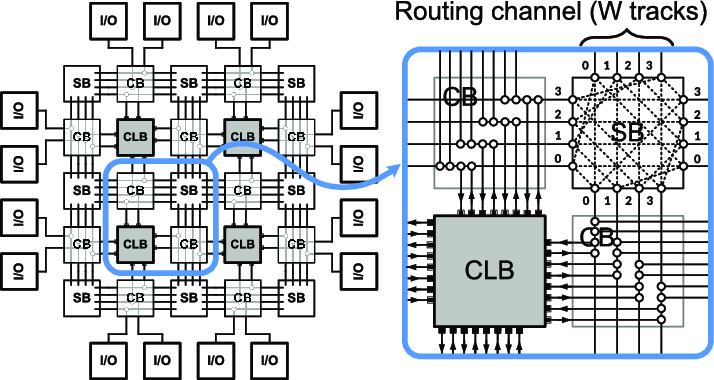
\includegraphics[width=\textwidth]{figures/clb.png}
\caption[Generic FPGA hardware architecture]{Generic FPGA hardware architecture. Depicted is the basic structure of a CLB and the interconnecting network.}
  \label{fig:clb}
\end{figure}

\pagebreak

Unlike general purpose systems such as CPUs or GPUs, this architecture allows the design of algorithms with arbitrary calculation widths, resulting in very good performance when processing images, both in power and time (see \autoref{fig:op_watt}).

\begin{figure}[h!]
\centering
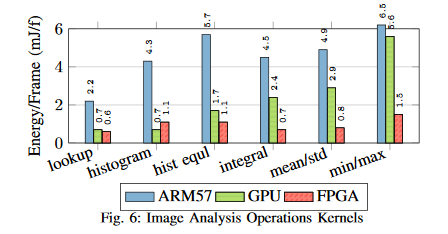
\includegraphics[width=\textwidth]{figures/op_watt.png}
\caption[Efficiency comparison between CPU, GPU and FPGA for image processing]{In image analysis kernels  such  as  lookuptable, histogram, and histogram equalization, the energy/frame consumption  of  the  FPGA  achieves  an  average  reduction  of 1.2× compared  to  the  GPU.  For  kernels  with  more branching  conditions  and  complex  memory  access  patterns, such as integral image, mean/std, and min/max locations, the FPGA’s  implementation  achieved  an  average  reduction  ratio of 3.5× compared to the GPU\cite{ochoa-ruiz_high-level_2012}}
  \label{fig:op_watt}
\end{figure}

\pagebreak

The space environment not only limits avaiable power, it also presents a challenge in the form of ionizing radiation. As this is one of the target markets for FPGA manufacturers, there are numerous chips with the necessary radiation resistance certifications.
%http://microelectronics.esa.int/techno/fpga_002_01-0-4.pdf
%https://amstel.estec.esa.int/tecedm/website/biblio/AFLDCIS2010.pdf
\\
ASICs provide the same design flexibility as FPGAs but their manufacturing rigidity allows them to achieve better performance by only including the specific design logic. However, their cost in small to medium scale projects is prohibitive. In addition, the flexibility of FPGAs allows reconfiguration already in the ship, allowing the use of different algorithms or bug fixes.
%https://iopscience.iop.org/article/10.1088/1742-6596/1195/1/012012/pdf
%https://amstel.estec.esa.int/tecedm/website/stag_ygt/Boada.pdf
\\
\\
In addition, since most algorithms share certain basic operations such as storage or high-precision arithmetic operations, FPGA manufacturers include certain prefabricated blocks in the circuit, which although remove some flexibility, provide better performance than the same logic in CLBs. These blocks are mainly RAM blocks and DSPs that allow a variety of operations, including multiplication or accumulation. This heterogeneous architecture (see \autoref{fig:heterogenea}) allows the implementation of high-performance algorithms where it would be impossible using only logic and brings FPGAs a little closer to the scope of ASICs \cite{zhou_efficient_2013}.
\begin{figure}[h!]
\centering
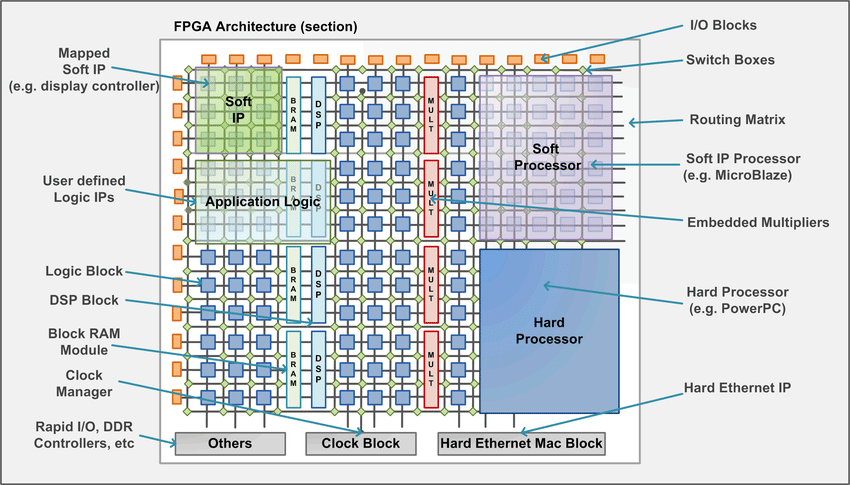
\includegraphics[width=5.7in]{figures/FPGA_heterogenea.png}
\caption[Overview of an heterogeneous FPGA]{Heterogeneous FPGA, depicting general configurable resources, DSPs, BRAMs and soft (implemented in logic) and hard (prefabricated) CPUs}
  \label{fig:heterogenea}
\end{figure}
\pagebreak
\\

\subsection{Hyperspectral imagery}
A standard camera captures images composed of 3 distinct light bands, which we humans perceive as red, green and blue. Their spectra correspond to high wavelengths between $564$ and $580 nm$ for red, mediums between $534$ and $545 nm$ for green and short ones between $420$ and $440 nm$ for blue. The rest of the spectra are invisible to our eyes.
\\
However, hyperspectral cameras capture information in many more spectra, both between the visible bands and outside them, allowing a much wider spectrum to be analyzed. These bands are usually shown as a third dimension, giving the name of hypercube to these images (see \autoref{fig:cube}).
\\
\\
\begin{figure}[h!]
\centering
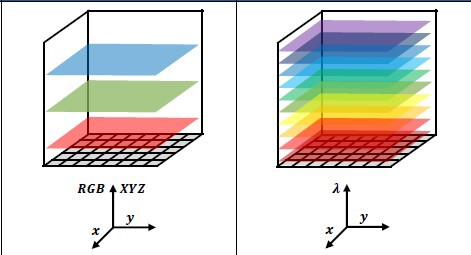
\includegraphics[height=2in]{figures/rgb_vs_hsi.jpeg}
\caption[Comparison between a standard and a hyperspectral image]{Comparison between the three bands of a standard camera and the multiple bands of an hyperspectral camera}
  \label{fig:cube}
\end{figure}
\\
%url{https://towardsdatascience.com/what-are-hyper-spectral-images-a5de5d9fa91}
\\
\\
These spectra or bands form together a hyperspectral signature for each material, which when compared with aerial images allow the recognition of different types of vegetation, mineral deposits or contaminants on the Earth's crust (see \autoref{fig:cuprite}).
\\
\\
\begin{figure}[h!]
\centering
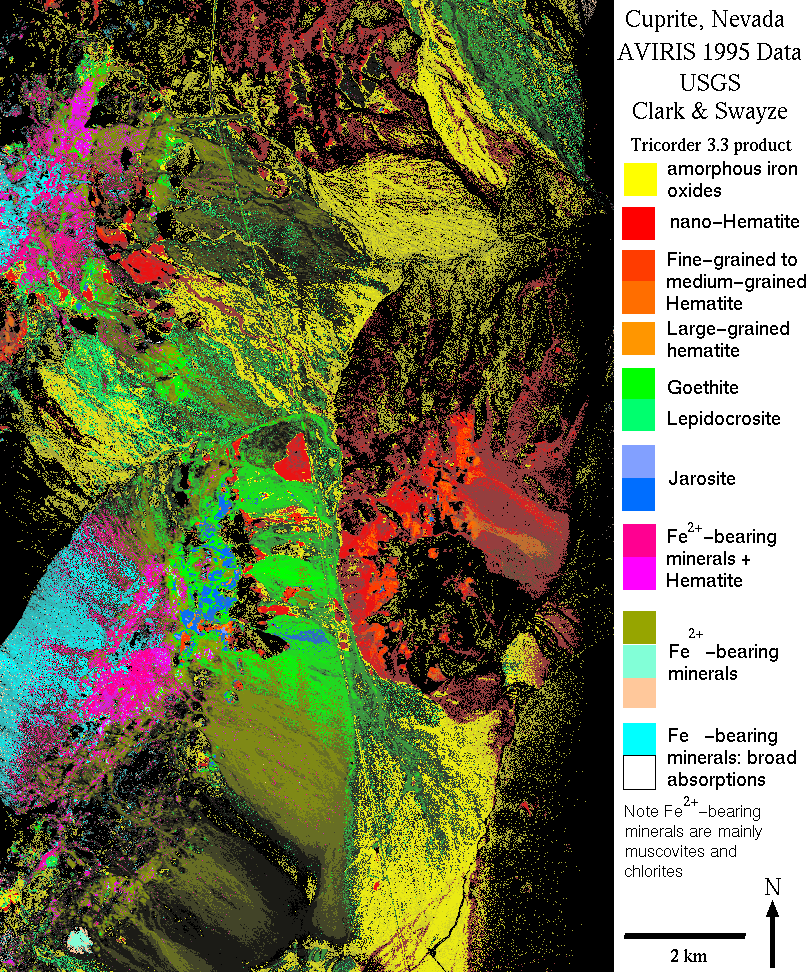
\includegraphics[height=6in]{figures/cuprite.png}
\caption[AVIRIS image of Cuprite, Nevada]{The map shown is a mineral map from an AVIRIS scene flown over Cuprite, Nevada, in 1995 \citep{noauthor_aviris_nodate}. It shows the mapping of many different minerals}
  \label{fig:cuprite}
\end{figure}
\clearpage


In this type of images, we can talk about two types of resolutions: spatial and spectral, the latter being unique in this type of cameras. Spatial refers to the number of meters covered by each pixel, so for the same camera you can change from one image to another. The spectral resolution refers to the separation between different wavelengths measured in a given range, that is, the more bands captured in a lower range, the higher the spectral resolution will be \cite{amigo_chapter_2020}.
\\

As technology advances, these resolutions continue to increase highlighting the need for commensurate processing systems.

\subsection{Anomaly detection}
In theory, a material should always have the same spectral signature. In practice, the captured signature will never be the same as the one measured in a laboratory because of differences in lighting, atmospheric effects, noise, etc. resulting in spectral variation for similar materials \cite{borsoi_spectral_2020}.

This has led to the development of algorithms that instead of classifying observations according to their signature, seek to classify the observations into unusual or anomalous materials and background. This assumes that the material -the target- is spectrally distinguishable from the background. The background is derived globally from the image assuming that it follows a normal distribution.

%\url{http://downloads.hindawi.com/journals/jece/2012/425947.pdf}\\
%\url{http://downloads.hindawi.com/journals/jece/2012/628479.pdf}\\
%\url{http://downloads.hindawi.com/journals/jece/2012/103286.pdf}\\
%\url{http://downloads.hindawi.com/journals/jece/2012/162106.pdf}

\subsubsection{RX algorithm}
The Reed-Xiaoli anomaly detector algorithm is a common algorithm that serves as the basis for many others.%\url{http://downloads.hindawi.com/journals/jece/2012/162106.pdf}\url{http://downloads.hindawi.com/journals/jece/2012/425947.pdf}\\%https://www.researchgate.net/publication/224166337_A_tutorial_overview_of_anomaly_detection_in_hyperspectral_images
%\url{http://downloads.hindawi.com/journals/jece/2012/162106.pdf}

The algorithm is defined by the following expression \cite{molero_fast_2011}:
\\
\[\delta ^{RX}(x) = (x-\mu)^{T}K^{-1}(x-\mu)\]

\paragraph{}
\phantomsection
\label{mayor}
Where $x$ is a hyperspectral pixel, a vector of size equal to the number of bands, $\mu$ is the mean of each band and $K$ is the covariance matrix. It is important to say that the results generated by the algorithm are grayscale 2D images. The anomalies have a high value, so the first anomaly corresponds to the pixel with the highest value, and so on.

\subsubsection{Other methods}
Apart from the RX algorithm, there are other methods for detecting anomalies, although a notable number of them are based on RX.

\subsubsection{Subspace methods}
Subspace methods are global and apply principal component analysis (PCA) or singular value decomposition (SVD) to the hypercube. The first PCA/SVD bands are supposed to be the background and are removed differently by each method. Not removing enough bands means that the anomalies can be lost in the background noise and removing too many would lead the anomalies to disappear. The determination of the correct number of bands to be removed is still under study \cite{borghys_hyperspectral_2012}.

\paragraph{Subspace RX}
In this method, the RX algorithm is applied to a limited number of PCA bands. The first components are discarded.

\paragraph{RX after orthogonal subspace projection \cite{matteoli_tutorial_2010}}
In this method, the first PCA/SVD components define the subspace of the background and the data is projected onto an orthogonal space before applying XR.

\paragraph{RX after partialling out the clutter subspace \cite{lo_hyperspectral_2009}}
In this method, clutter effect on a pixel is discarded component wise taking each of its spectral components as a linear combination of its high variance principal components. The RX algorithm is applied to the results.

\paragraph{Complimentary subspace detector \cite{chein-i_chang_anomaly_2002}}
This algorithm is not based on RX. In CSD, the principal components with higher variance are used to define the subspace of the background and the other PCs to define the subspace of the target. The pixel is then projected onto the two subspaces and the result is the difference between them.

\subsubsection{Local methods}
In the local methods the background is derived from the neighboring pixels or surroundings of the pixel under test (PUT). Two windows are defined, a guard and an exterior, and the neighbors are the pixels that are between these two. Sometimes, for example in local RX, a third one is used where the covariance of the background is calculated in a window larger than the average of the background (see \autoref{fig:ventana}).

\paragraph{Quasi-local RX \cite{gorelik_target_2012}}
Quasi-local RX is a compromise between global RX and local RX, where the global covariance matrix is decomposed using eigenvector/eigenvalues. The eigenvectors are maintained, but the eigenvalues are replaced by the maximum local variance, resulting in lower detector scores in areas with high variance.

\begin{figure}[h!]
\centering
%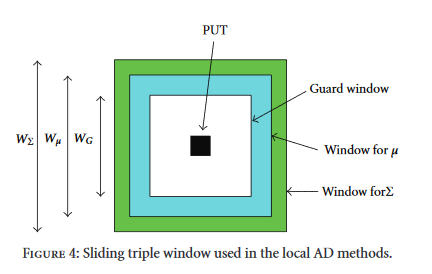
\includegraphics[height=2.5in]{figures/ventana.png}
\hspace*{100pt}%
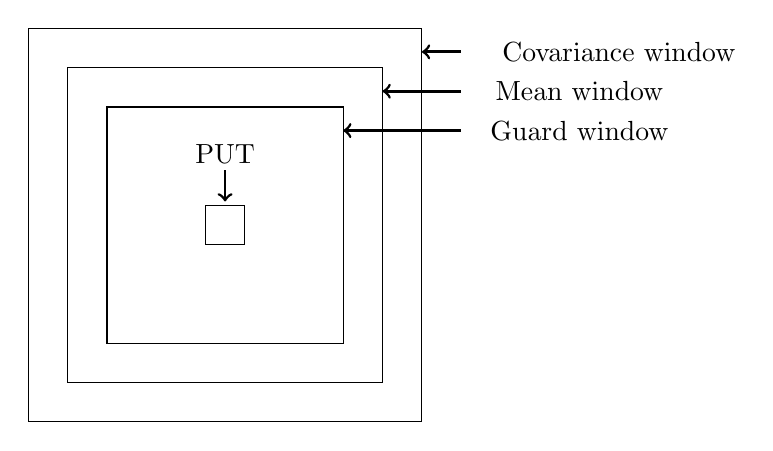
\begin{tikzpicture}
        \draw (0,0) rectangle (5,5);
        \draw[arrows=<-,line width=1pt](5,5-.3)--(5.5,5-.3);
        \draw (7.5,5-0.3) node{Covariance window};
        
        \draw (.5,.5) rectangle (4.5,4.5);
        \draw[arrows=<-,line width=1pt](4.5,4.5-.3)--(5.5,4.5-.3);
        \draw (7,4.5-0.3) node{Mean window};
        
        \draw (1,1) rectangle (4,4);
        \draw[arrows=<-,line width=1pt](4,4-.3)--(5.5,4-.3);
        \draw (7,4-0.3) node{Guard window};
        
        \draw (2.25,2.25) rectangle (2.75, 2.75);
        \draw[arrows=<-,line width=1pt](2.5, 3-.2)--(2.5, 3.2);
        \draw (2.5, 3.4) node{PUT};
    \end{tikzpicture}
\caption[Sliding window used in some algorithms]{Sliding triple window used in the local AD methods.}
  \label{fig:ventana}
\end{figure}

\subsubsection{Segmentation based methods}
In complex scenes it is difficult to assume that the background will be defined by a normal distribution, so methods have been developed to separate it into different classes.

\paragraph{Class-Conditional RX \cite{lo_hyperspectral_2008}}
In this method the image is first segmented and the covariance and mean matrix calculated for each of these classes. Each pixel will correspond to the class in which its RX value is lower.

There are more methods within those based on segmentation, from those using stochastic functions such as Method Based on Multivariate Normal Mixture Models to methods based on Self-organizing maps.
\pagebreak
\subsection{Comparing floating and fixed point}
\label{makereference}

In computer systems, there are two numerical representations for real numbers, fixed and floating point. They have different arithmetic, which gives them different range and resolution with the same number of bits. Therefore, there are certain applications or platforms more akin to one of them. For example, the ability of floating point numbers to contain in the same number of bits both very large and very small numbers and to adjust their resolution accordingly is very attractive from the programmer's point of view but the simplicity of fixed point operations allow their use in small microcontrollers or to save resources in FPGAs (see \autoref{fig:fp}).
\begin{figure}[h!]
\centering
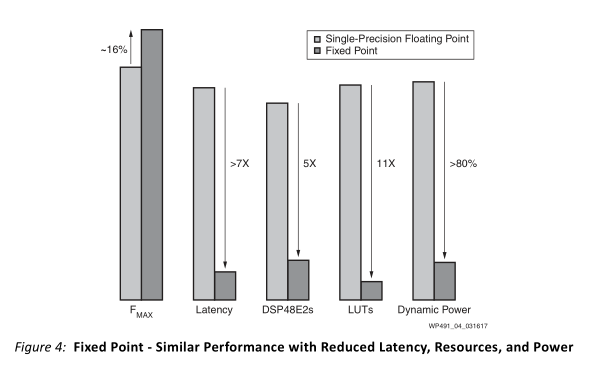
\includegraphics[height=3.5in]{figures/fp_vs_fp.png}
\caption[Performance comparison between fixed and floating point]{A FIR filter, originaly implemented as a single-precision floating-point filter and converted to fixed-point. The fixed-point design shows both resource reduction and latency improvements}
  \label{fig:fp}
\end{figure}
\\
Due to the high complexity of hyperspectral image analysis, current FPGAs have little capacity to implement some of these algorithms. Therefore, one of the objectives of this work is to perform two parallel implementations, one in floating point and another one in fixed point and compare their results.

\pagebreak
\section{Project plan}
First, an algorithm and a hardware platform are chosen. Desirably, this algorithm should be known and commonly found in the literature.
\\
This algorithm will be implemented in software and this implementation tested with real images against existing software such as ENVI or Spectral Python.
\\
The different algorithm stages will then be optimized for a hardware architecture and the transformation of the algorithm from floating point to integer or fixed point logic will be studied.
\\
This transformation requires design decisions that sacrifice precision with the goal of saving hardware resources, so the underlying hardware will have to be considered.
\\
Subsequently, a hardware validation of the design will be realized.
\\
Finally, a study will be carried out on the accuracy of the results obtained.
\\
\\
    \begin{figure}[h!]
    \begin{tikzpicture}
      \GanttHeader{\textwidth-0.6cm}{2ex}{3.5cm}{10}
      \Task{1}{Research algorithms}{0.5}{1}
      \Task{2}{Software impl.}{1}{4}
      \Task{3}{Model hardware}{2}{4.5}
      \Task{4}{Hardware impl.}{6}{2}
      \Task{5}{Test and validation}{7}{2}
      \Task{6}{Report results}{8.5}{1}

      %\arrowwhereboxesoverlap[thick,red,->]{1}{2}
      %\draw [blue,dashed,very thick,->] (2b) -- ++ (0.2,0) |- (4a);
\end{tikzpicture}
    \caption[Gantt diagramm of this work]{Gantt diagram with an overview of months and tasks}
    \label{fig:gantt}
    \end{figure}
